\documentclass[titlepage, a4paper, 11pt]{scrartcl}

%too much whitespace otherwise
\usepackage[left=2cm,right=2cm,top=2cm,bottom=2cm]{geometry}

% Grafik Pakete
\usepackage{graphicx,hyperref,amssymb}

% Ordner für Grafiken
\graphicspath{ {./Grafiken/} }

\usepackage[utf8]{inputenc}
\usepackage[german]{babel}
\usepackage[T1]{fontenc}
\usepackage{amsmath}
\usepackage{amsfonts}
\usepackage{amssymb}
\usepackage{graphicx}

\usepackage{caption}
\usepackage{subcaption}

% Header and Footer
\usepackage{fancyhdr}

\pagestyle{fancy}
\fancyhf{}
\rhead{Lückert, Neudecker, Schnoor}
\lhead{AR Exhibition - Dokumentation}

\title{AR Exhibition - A LiDAR powered AR Application}
\author{Marlon Lückert \\ Bachelor of Science \\ \href{mailto:marlon.lueckert@haw-hamburg.de}{marlon.lueckert@haw-hamburg.de} 
\and Julius Neudecker \\ Bachelor of Science \\ \href{mailto:julius.neudecker@haw-hamburg.de}{julius.neudecker@haw-hamburg.de}
\and Vincent Schnoor \\ Bachelor of Science \\ \href{mailto:vincent.schnoor@haw-hamburg.de}{vincent.schnoor@haw-hamburg.de} }
\date{November 2020}


\begin{document}

  \maketitle

  \tableofcontents

  \begin{abstract}
    Here goes some nice abstract, outlining the project and its challenges briefly...
  \end{abstract}

  %1. - Beschreibung des Projektes, Ziel, Forschungsfragen, Zielgruppe
  %
  %2.1 - Technische Umsetzung Beschreibung, Skizzen, Bilder, …
  %2.2- Recherche, Literaturübersicht, State of the Art Technik, Diskussion der existierenden Ansätze mit der eigenen Lösung und die innerhalb des Projektes zu meisternden Herausforderungen (W-Fragen)
  %
  %3.1 - User Research, gewählte Methoden, warum habt ihr die gewählt, wie habt ihr sie für eure Evaluation eingesetzt?
  %3.2- Analyse Nutzerbefragung
  %
  %4. Schlussfolgerungen aus 2 und 3
  %5. Ausblick für Weiterentwicklungen …
  %6. Appendix in Form von Daten

  \section{Projektbeschreibung}
  % Wovon handelt das Projekt? Wie ist es entstanden? Warum ist es interessant?
  Das Projekt \textit{ARExhibition}, welches im Rahmen des Projektes \textit{XRchitecture} entstanden ist macht das Ausstellen digitaler Modelle und Medien einfacher. Mit nur wenigen Klicks können 3D-Modelle, Bilder und Videos aus einem hierfür entwickelten Content-Management-System (CMS) in AR platziert und gespeichert werden. Die so entstandenen AR-Szenen können von Besuchern über einen Marker geladen und betrachtet werden.\\
  Diese Ausstellungen können bspw. von Hochschulen und anderen Bildungsinstituten genutzt werden um Projekte der Studierenden und Schüler auszustellen.
  \subsection{Projektziel}
  % Was soll erreicht werden?
  Ziel des Projektes ist es, die Darstellung medialer Inhalte der Hochschule und anderer Lehrinstitute einfacher zu gestalten und eine Oberfläche für die Studenten der HAW zu schaffen um ihre im Semester erstellten 3D-Modelle, Bilder und Videos an einem zentralen Ort zu speichern und mit anderen Studierenden zu teilen.
  \subsection{Zielgruppen}
  % Welche Zielgruppen werden mit dem Produkt angesprochen und warum?
  Für unser aus zwei Teilen bestehendes Projekt gibt es zwei Zielgruppen.\\
  Die erste Zielgruppe besteht aus den Studenten der HAW welche das Content-Management-System zum einfachen Teilen ihrer Arbeiten nutzen können. Die Projekte anderer Studiengänge und Fakultäten können so leichter eingesehen werden. Außerdem können die Arbeiten anderer Studenten heruntergeladen und für eigene Studienprojekte verwendet werden.\\

  Bildungsinstitute wie die HAW Hamburg und Bildungsstätten wie Museen bilden die zweite Zielgruppe. Für bspw. die HAW Hamburg wird die Ausrichtung von Ausstellungen der Studentenprojekte vereinfacht, da Räume interaktiver und sinnvoller mit digitalen Medien gefüllt werden können. Wo vorher 3D-Objekte auf PC Bildschirmen betrachtet werden mussten, können diese mithilfe der App als Teil des Raumes betrachtet und mit ihnen interagiert werden. Museen und Ausstellungen können durch die App ihr Repertoire an Kunst und Objekten erweitern, da virtuelle Bilder und Objekte einfach ausgestellt werden können. Die Inhalte können genau wie vom Kurator gewollt platziert werden und erscheinen dem Besucher in der gewollten Position, Rotation und Größe.

  \section{Technische Umsetzung}
  % Wie funktioniert die App, bzw. das CMS? Welche Software/Hardware Einheiten werden verwendet?
  Das Projekt besteht aus zwei gleich großen Bestandteilen: einem Content-Management-System, welches für die Bereitstellung des Inhalts der App und als Speichermedium studentischer Projekte dient und der App, welche die Platzierung virtueller Inhalte in einem Raum in AR ermöglicht.\\
  Im Folgenden wird die technische Umsetzung des CMS und der App erläutert. Dabei wird auf bereits existierende ähnliche Produkte eingegangen und wie unser Projekt sich von diesen abgrenzt. Verschiedene Ansätze der Umsetzung werden diskutiert und miteinander verglichen und die Schwierigkeiten der Umsetzung werden erläutert.
  \subsection{Stand der Forschung}
  % Welche Literatur liegt dem Projekt zugrunde, bzw. welche anderen Produkte/Projekte? Inwiefern grenzt sich unser Projekt von diesen ab?
  \subsection{Content-Management-System}
  \subsubsection{Aufbau der Datenbank}
  \subsection{AR App}
  \subsubsection{Verwendung von 3D-Modellen}
  Da die Platzierung von 3D-Modellen ein Hauptbestandteil der App ist, wurde ein großer Fokus auf das Dateiformat der 3D-Modelle gelegt. Die dynamische Verwendung der Modelle in der App sollte möglichst einfach und problemlos sein.\\ 
  Aus diesem Grund wurden die verschiedenen von Unity unterstützten Dateiformate miteinander verglichen, um die im Dateiformat unterstützten Funktionalitäten und die Qualität der Darstellung in der App zu vergleichen.\\
  Unity unterstützt nativ die folgenden Dateiformate:
  \begin{itemize}
  \item FBX
  \item DAE (Collada)
  \item DXF
  \item OBJ
  \end{itemize}
  Da die meisten Studenten Blender als 3D-Modelling Tool ihrer Wahl nutzen wurde ein Vergleich der in Blender möglichen Export-Dateiformate und der in Unity unterstützten Formate gemacht. Blender exportiert 3D-Modelle unter anderem als FBX und OBJ, welche ohne großen Aufwand in Unity importiert werden können.\\
  Der Nachteil dieser Formate ist, dass die Materialien und Texturen als externe Dateien in einem getrennten Ordner exportiert werden. Für die direkte Verwendung in Unity kein Problem erschwert dies jedoch das Zwischenspeichern in unserem Content-Management-System. Weiterhin werden \glqq Faces\grqq, Flächen eines 3D-Modells, mit mehr als 5 \glqq Vertices\grqq, Eckpunkten, nicht unterstützt und somit in Unity nicht dargestellt. Bei nicht komplett sauber erstellten 3D-Modellen können so unschöne Lücken im Modell entstehen die unerwünscht sind.\\
  Aus diesem Grund wurde das von der Khronos Group entwickelte und in Blender integrierte GLTF 2.0 Format auf seine Verwendbarkeit in Unity untersucht. GLTF speichert sämtliche Daten eines 3D-Modells, darunter auch Materialien und Animationen, in einer einzigen, auf dem JSON-Dateiformat basierenden Datei ab. Das Dateiformat ist extrem robust und speichert jegliche Geometrie eines 3D-Modells ab. Der Nachteil des GLTF-Formates ist allerdings, dass dieses erst ab der Blender Version 2.81 unterstützt und erst ab 2.83 richtig implementiert ist. Alte Blender Modelle müssen demnach auf eine höhere Blender-Version gebracht und dort exportiert werden. Weiterhin unterstützt Unity, wie in der Auflistung oben zu sehen, das Dateiformat GLTF 2.0 nicht nativ, weshalb zusätzliche Bibliotheken benötigt werden um die Dateien nutzen zu können.\\
  Eine dieser und die in unserem Projekt verwendete Bibliothek ist die \textit{GLTFUtility} Bibliothek des GitHub-Nutzers \textit{Siccity}. \textit{GLTFUtility} unterstützt den Import und Export von GLTF Dateien in Unity während der Laufzeit, was für unser Projekt von elementarer Bedeutung ist, da die 3D-Modelle beim Starten der App nicht bereits vorliegen, sondern während der Laufzeit der App dynamisch geladen und verwendet werden.\\

  Der Vergleich der drei untersuchten Dateiformate hinsichtlich Qualität zeigte, dass die Darstellung von GLTF-Modellen gegenüber FBX- und OBJ-Modellen besser ist (siehe Abbildungen x, y und z). Die von Blender exportierten Materialien werden im GLTF-Format, durch die bessere Unterstützung diverser Material-Eigenschaften, besser dargestellt.\\

  Aus diesen Gründen, der besseren Darstellung der 3D-Modelle in Unity, die robustere Geometrie-Darstellung und der Export in einer einzigen Datei, entschieden wir uns dazu GLTF als einziges Dateiformat für die Verwendung innerhalb der App zu verwenden.
  \subsubsection{Export-Anforderungen an 3D-Modelle}
  Die im Laufe des Projektes erstellten Anforderungen an den Export der 3D-Modelle hinsichtlich ihrer Material-Eigenschaften und Animationen beziehen sich ausschließlich auf den Export in der 3D-Modelling-Software Blender.\\

  Die in Blender erstellten Materialien weisen mit zunehmender realitätsnähe eine steigende Komplexität auf. Aus diesem Grund mussten bestimmte Anforderungen an den Export von 3D-Modellen aus Blender gestellt werden, um die korrekte Darstellung in der von uns entwickelten App zu gewährleisten. Die folgenden Anforderungen gelten für den Export von 3D-Modellen aus Blender um die Darstellung in unserer App zu gewährleisten.\\

  \textbf{Meshes:}\\
  GLTF unterstützt den Export von jeglicher Geometrie des Meshes. Dabei ist die Anzahl der Vertices eines Faces irrelevant, da Quads und N-Gons beim Export automatisch in Triangles umgewandelt werden.\\
  Kurven und andere \glqq Nicht-Mesh\grqq Daten werden nicht übernommen uns müssen vor dem Export in Meshes umgewandelt werden.\\

  \textbf{Materialien:}\\
  GLTF unterstützt die folgenden Material-Eigenschaften beim Export:
  \begin{itemize}
  \item Base Color
  \item Metallic
  \item Roughness
  \item Baked Ambient Occlusion
  \item Normal Map
  \item Emissive
  \end{itemize}
  Texturen werden als Base Color problemlos unterstützt. Bei Roughness und Metallic Texture-Maps müssen einige Einstellungen vor dem Export getroffen werden. Bei einer Textur erwartet GLTF die Metallic-Werte kodiert im B-Farbchannel, während die Roughness-Werte im G-Farbchannel kodiert sind. Das Node-Setup in Blender sollte demnach folgendermaßen aussehen:\\
  %Bild einfügen
  Wurde das Node-Setup nicht angepasst wird versucht beim Export die relevanten Daten auszulesen, was mitunter zu längeren Exportzeiten führen kann.\\
  Baked Ambient Occluion, Normal Maps und Emissive Materials werden problemlos unterstützt und müssen nicht weiter angepasst werden.\\

  \textbf{Animationen:}\\
  Animationen im GLTF-Format zu exportieren ist nicht kompliziert. Folgende Animationstypen werden nativ beim Export unterstützt:
  \begin{itemize}
  \item Keyframes (Translation, Rotation, Scale)
  \item Shape Keys
  \item Armatures/Skinning
  \end{itemize}
  Animationen anderer Eigenschaften wie Licht oder Materialien werden ignoriert.\\
  Wenn das 3D-Modell nur eine Animation hat gibt es bei der Verwendung in Unity keine Probleme. Probleme entstehen wenn das 3D-Modell aus mehreren Einzelteilen besteht die jeweils eigene Animationen haben, da die Animationen in Unity im Legacy Animation-System abgespielt werden müssen, welches nur eine Animation zur Zeit unterstützt. Aus diesem Grund müssen mehrere Animationen einem NLA Track hinzugefügt werden. Dieser dient quasi als Animations-Controller, welcher die einzelnen Animationen zu einer einzigen Animation zusammenfasst und die verschiedenen Objektteile bewegt.\\
  Objekt-Constraints, wie \glqq Copy Location\grqq können ebenfalls exportiert werden, wenn diese vorher in Keyframes umgewandelt wurden.\\
  Die letzte Anforderung beim Export von 3D-Modellen mit mehreren Einzelteilen und Animationen ist, dass es nur \textbf{ein} Parent-Objekt geben darf. Dies kann ein leeres Objekt sein, da dies für die Hierarchy in Unity und die Verwendung der Animationen relevant ist.\\

  Wenn diese Anforderungen eingehalten werden können Blender-Modelle exportiert und in unserer App verwendet werden.

  \subsubsection{Speichern und Wiederherstellen der Einrichtung eines Raumes}

  Eine wichtige Funktion der App ist es, dass man in einem beliebigen Raum Assets platzieren kann und die Position, Rotation und Skalierung der einzelnen Assets speichern kann.
  Weitere User der App können dann die Assets exakt so wiederherstellen, wie sie vorab gespeichert wurden.

  Das zu lösende Problem besteht darin, dass beim Starten einer Augmented Reality Session immer ein neues Koordinatensystem angelegt wird.
  Der Ursprung dieses Koordinatensystems liegt immer bei der Position des AR Gerätes beim Start der App.
  Wenn nun also verschiedene Nutzer in unterschiedlichen Positionen im Raum starten, führt es dazu, dass die Assets nicht an der selben Position sind wie zuvor beim Speichern.
  
  Auf dieses Problem stößt man vor allem, wenn man sich mit dem Thema \textit{Indoor Navigation} beschäftigt. Hier muss die Navigation perfekt auf den realen Raum angepasst werden, damit die Navigation überhaupt funktionieren kann.
  Unsere App bewegt sich in der gleichen Problemdomäne, da die Assets für jeden Nutzer an der selben Position im realen Raum verankert sein müssen.

  Für dieses Problem gibt es unterschiedliche Lösungsansätze:

  \paragraph{GPS}
  GPS ist eine häufig eingesetzte Technologie für die Positionserkennung. Da es eine globale Standortermittlung ist, sind die Position für alle Nutzer ähnlich.
  Diese Technologie ist aber zu ungenau, vor allem beim Tracking innerhalb von Gebäuden. Auch ist es schwierig Stockwerke zu unterscheiden.

  \paragraph{Beacons}
  In der Indoor Navigation sind Beacons ein gute Möglichkeit einen Standort zu ermitteln. Beacons sind Geräte, die über Bluetooth eine Verbindung zu dem AR Geräte herstellen und so ermitteln können, wo sich ein Gerät befindet.

  \begin{figure}[h]
    \centering
    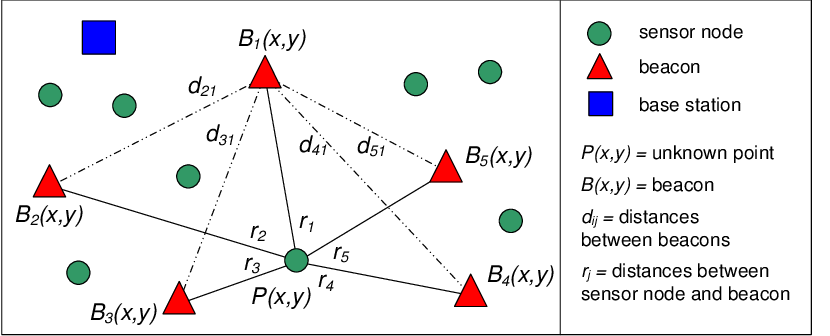
\includegraphics[width=.6\textwidth]{beacons}
    \caption{Positionsermittlung mit Beacons \cite{beaconNetwork}}
    \label{Beacons}
  \end{figure}

  In Abbildung \ref{Beacons} ist zu sehen, dass sich die Beacons (rot) an einer bekannten Position befinden. Die unbekannte Position (grün) wird durch die Abstände zu den einzelnen Beacons errechnet.

  Ein berühmtes Beispiel für den Einsatz von Beacons ist der Flughafen Gatwick in London. Hier wurden 2000 Beacons installiert, um die Indoor Navigation zu ermöglichen. \cite{GatwickA64:online} 
  Dieses System bietet eine Genauigkeit von +/- 3 Metern.
  
  Dies ist zu unganau für unsere Einsatzzwecke, da wir Assets mit der höchsten Genauigkeit platzieren und wiederherstellen möchten. Die Assets müssen sich genau in die Umgebung einbinden lassen.
  Ein Beispiel wäre die Platzierung eines 3D Objekts auf einem realem Sockel. Wenn die Ungenauigkeit bei mehreren Metern liegt, kann nicht gesichert sein, dass das 3D Objekt immer sich genau auf dem Sockel befindet.

  Des Weiteren müssen diese Beacons gekauft werden für etwas 5 - 20 Euro pro Stück und in jedem Raum installiert werden, der unsere App nutzen möchte.
  Es darf auch nicht vergessen werden, dass diese Geräte batteriebetrieben sind und somit nach 1-2 Jahren ein Wechsel der Batterien durchgeführt werden muss. 

  \paragraph{Image Markers}

  Eine weitere Möglichkeit um die Positionen der echten Welt mit der AR Welt zu synchronisieren sind \textit{Image Marker}. Meist werden Image Marker dazu genutzt 3D Objekte direkt mit einem Bild zu verankern, wie zum Beispiel bei AR Visitenkarten.
  Es ist aber auch möglich Objekte relativ zu einem Bild mit einem größerem Abstand zu platzieren. Denn wenn ein Bild mit einem AR SDK wie ARKit oder ARCore erkannt wird, wird die Position und Rotation des Bildes in der AR Session bestimmt.
  Wenn die Asset Positionen gespeichert werden, muss dies also relativ zu dem Image Marker passieren. Dazu muss immer ein Bild in einem Raum platziert werden und die Position des Bildes darf sich nicht mehr ändern, da sich sonst alle platzierten Assets ändern würden.
  Die Genauigkeit ist auf Millimeter genau. \cite{HowAugme98:online}
  
  Dennoch sinkt die Genauigkeit je weiter man sich von dem Marker entfernt.

  \begin{figure}[h]
    \centering
    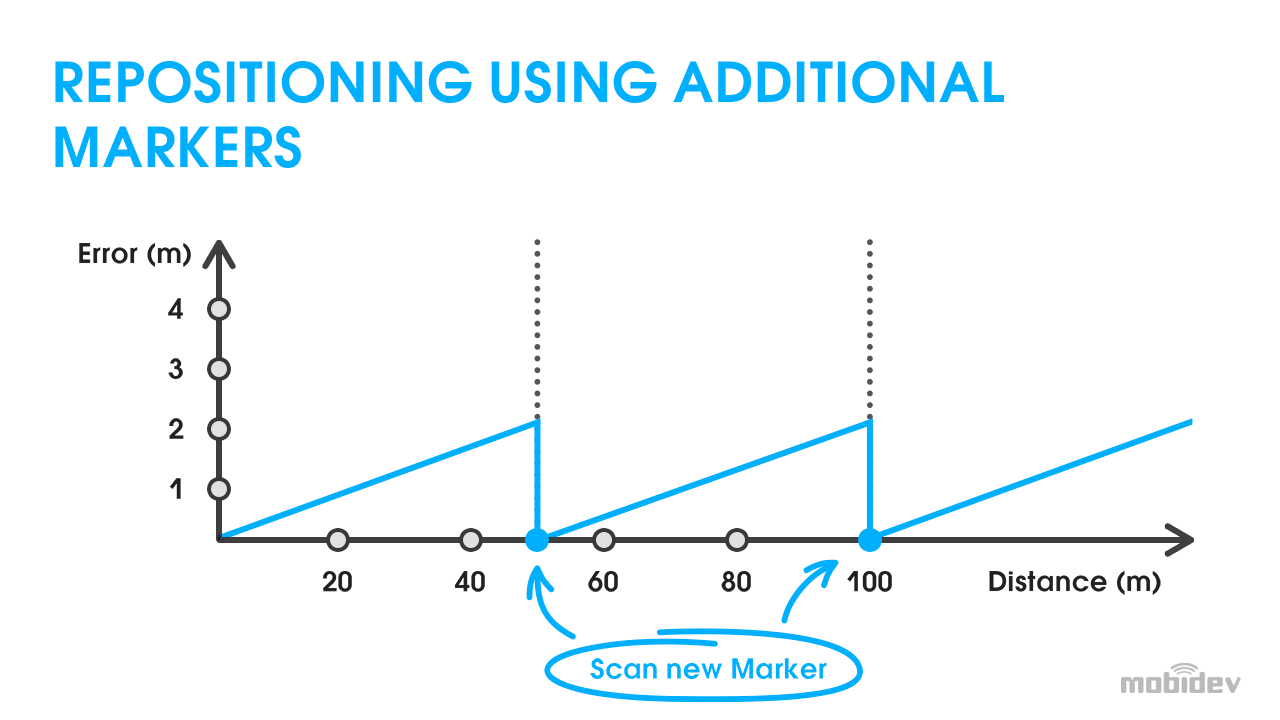
\includegraphics[width=.6\textwidth]{multi-marker}
    \caption{Repositionierung mit mehreren Image Markern \cite{HowAugme98:online}}
    \label{MultiMarker}
  \end{figure}

  In Abbildung \ref{MultiMarker} ist ein Beispiel einer Indoor Navigation zu sehen, die den Fehlerwert in Meter abhängig von der Distanz zu dem Image Marker zeigt.
  Hier wird mit mehreren Markern gearbeitet, um die Genauigkeit zu erhöhen.

  Der Vorteil dieses Ansatzes ist, dass die Genauigkeit im Bereich der Image Marker sehr hoch ist und die Marker günstig und einfach produziert werden können und ohne Strom betrieben werden.

  Der Nachteil ist, dass mit mehreren Markern gearbeitet werden muss, damit die Qualität dauerhaft gesichert werden kann. Auch muss bei der Positionierung des Markers darauf geachtet werden, dass sich die Position nicht mehr ändert.

  \paragraph{Visual Positioning System}

  Eine weitere Möglichkeit ist es eine Umgebung anhand von Referenzpunkten zu synchronisieren.
  Ein bekanntes Beispiel dieses \textit{Visual Positioning Systems} ist die AR Funktionalität von Google Maps.
  
  \begin{figure}[h]
    \centering
    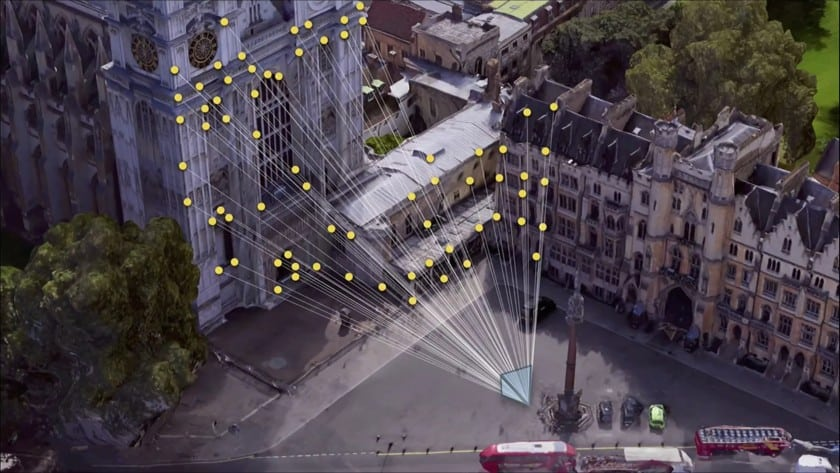
\includegraphics[width=.5\textwidth]{vps-google}
    \caption{VPS in Google Maps \cite{GoogleMa12:online}}
    \label{VPSGoogle}
  \end{figure}

  Bei Google Maps werden die Bilddaten der AR Kamera mit den Daten der Google Streetview Aufnahmen verglichen.
  Durch die Synchronisierung besonders markanter Stellen in der Umgebung (\textit{Feature Points}) kann die Position und Rotation in der realen Welt sehr genau wiederhergestellt werden.

  In Abbildung \ref{VPSGoogle} ist zu sehen wie anhand von Feature Points die Position der Kamera bestimmt wird.

  Das gleiche Prinzip kann auch auf Räume angewandt werden. Dazu werden zunächst die Feature Points aus einem Raum extrahiert und bei der Wiederherstllung wieder abgeglichen.

  \begin{figure}[h]
    \centering
    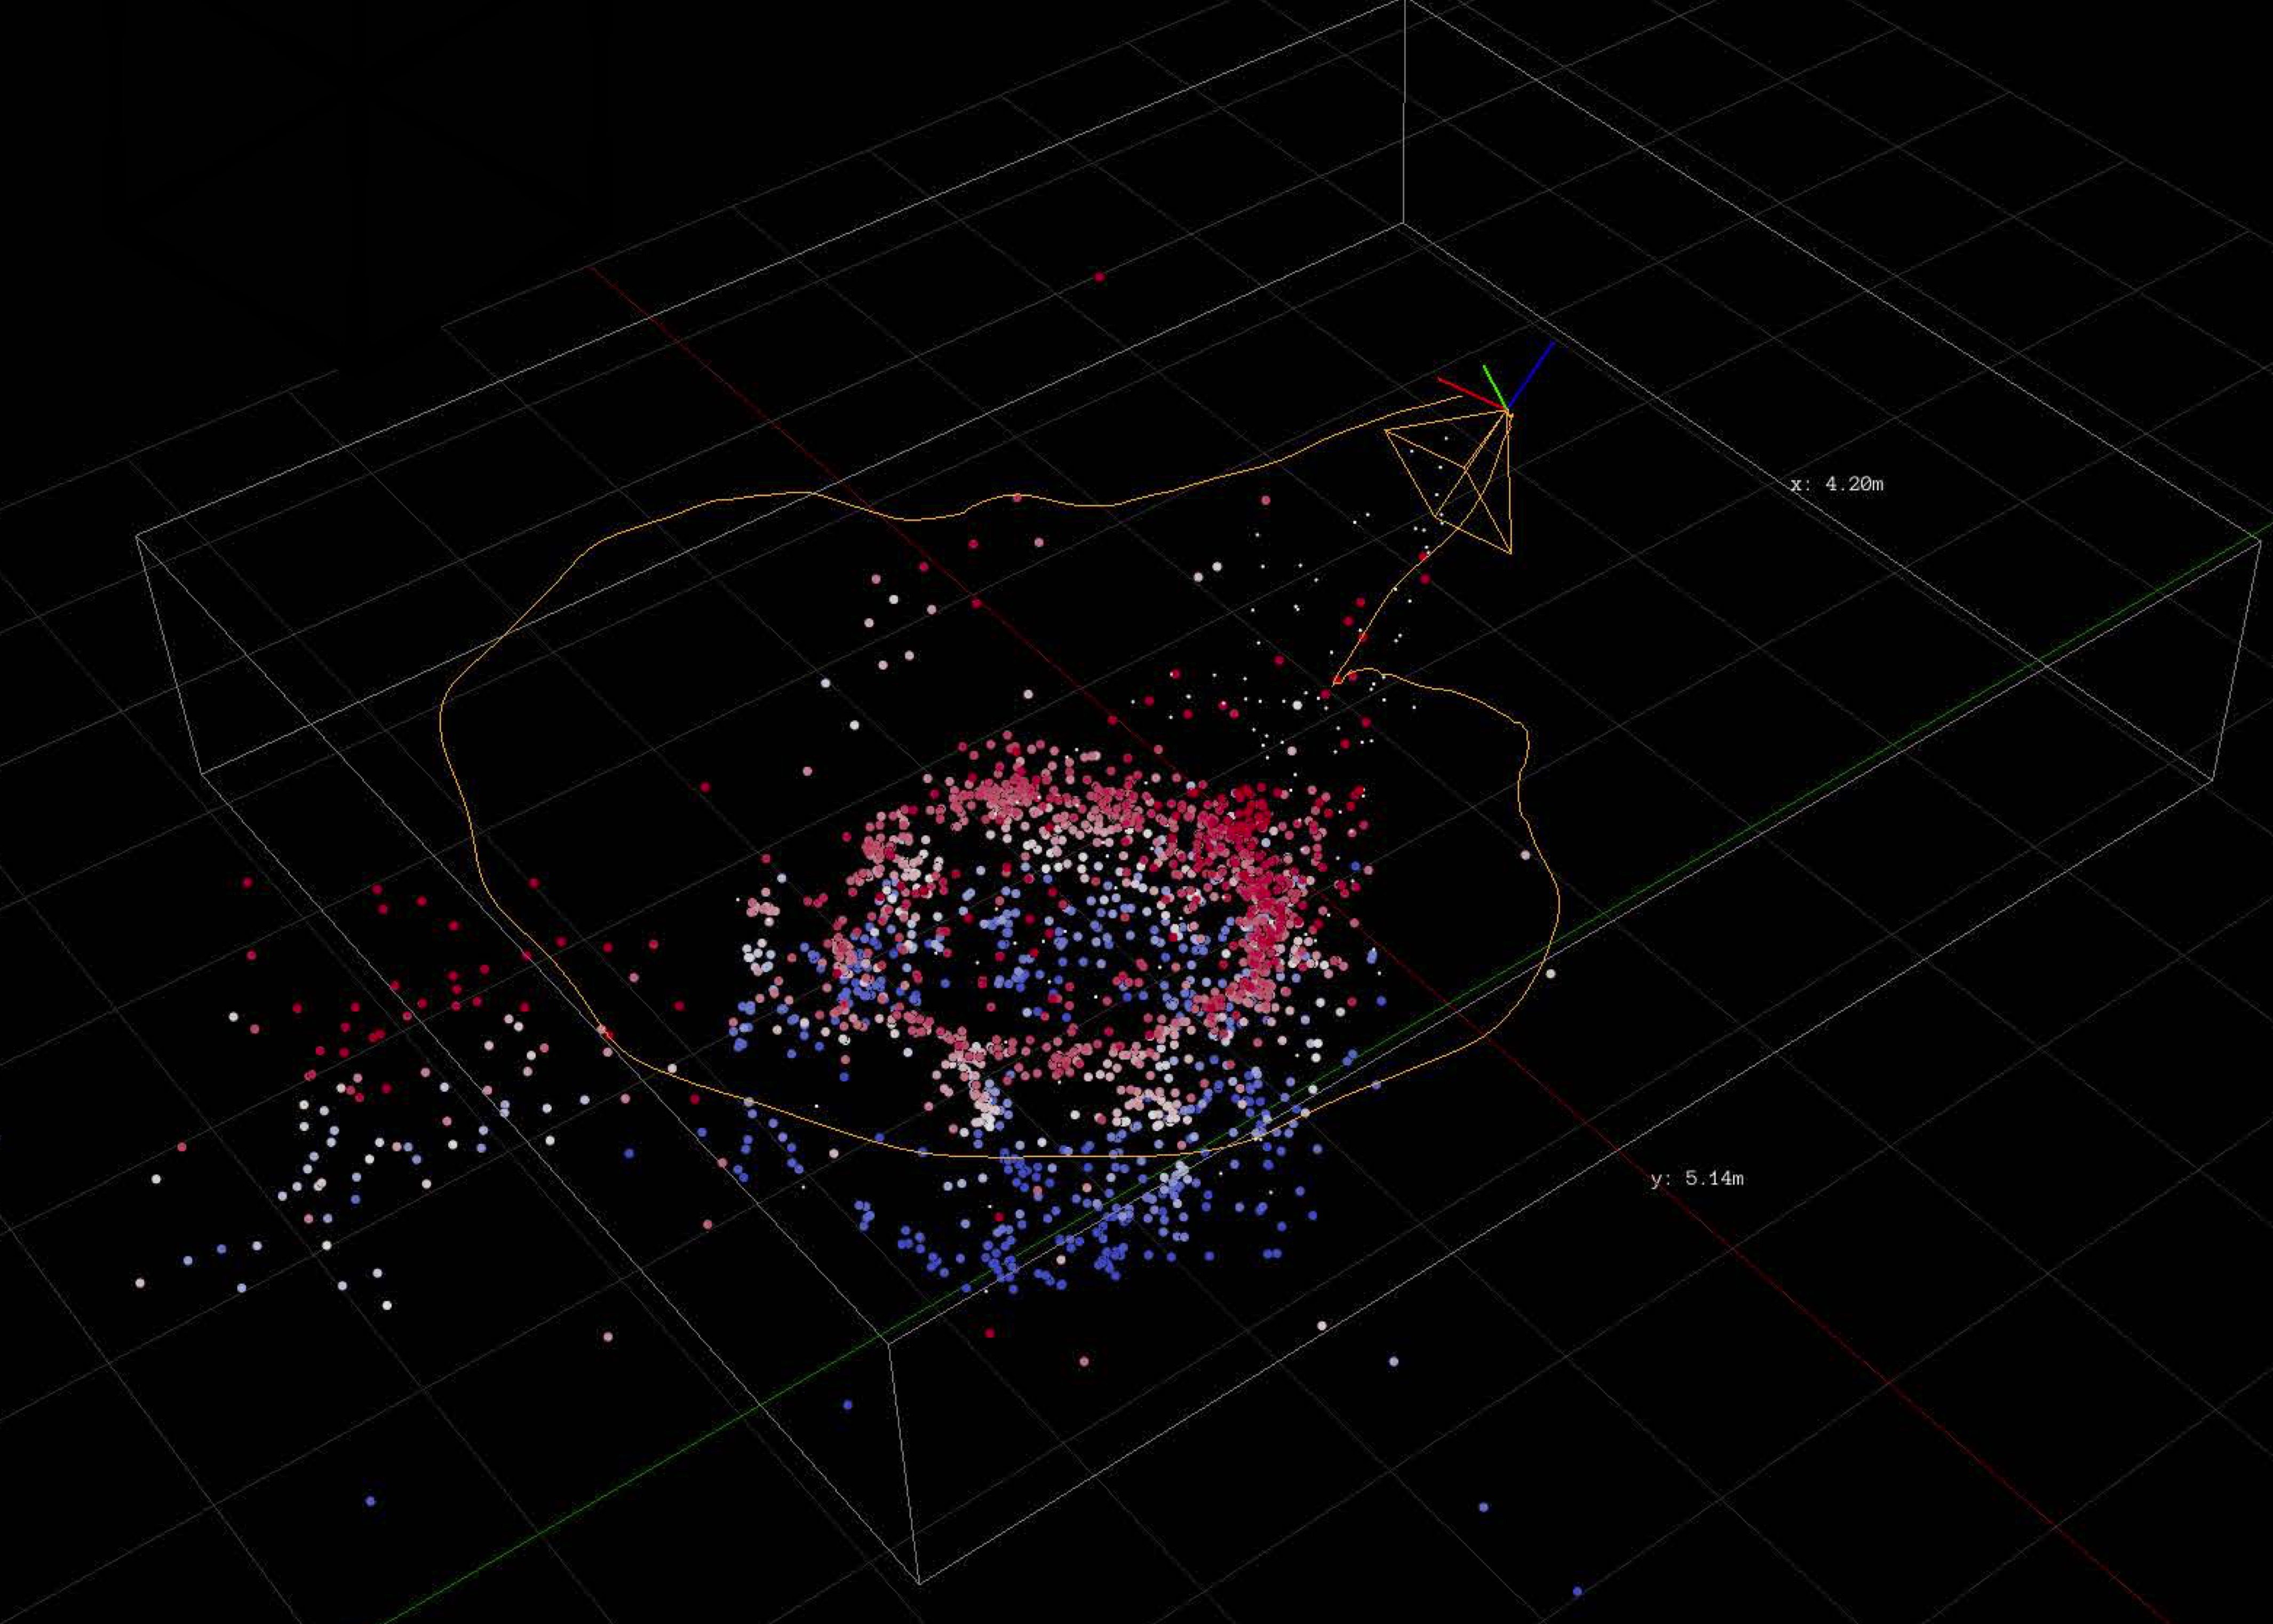
\includegraphics[width=.5\textwidth]{arworldmap-featurepoints}
    \caption{Feature Points}
    \label{FeaturePoints}
  \end{figure}

  In Abbildung \ref{FeaturePoints} ist zu sehen wie so eine Wolke von Feature Points im Raum aussehen kann.

  Der Vorteil dieses Verfahrens ist es, dass keine extenen Geräte oder Marker benötigt werden. Auch ist die Genauigkeit konstant hoch, da nicht nur ein Punkt (Image Marker), sonderen mehrere Punkte (Feature Points) gespeichert werden. Mit moderner Hardware wie LiDAR Sensoren, lässt sich die Performance noch weiter verbessern ohne die Technologie zu ändern.
  Der Nachteil ist, dass die Feature Points nicht abgeglichen werden können, wenn sich der Raum ändert, wenn also Gegenstände oder Möbel dem Raum hinzugefügt werden oder entfernt werden.
  Auch kann es bei großen Räumen zu einer großen Datenmenge kommen, wenn viele Feature Points extrahiert werden.

  \paragraph{Unsere Umsetzung}

  Bei der Auswahl des Verfahrens mussten wir zwischen \textit{Image Marker} und \textit{Visual Positioning System} abwägen.
  Wir haben uns für das \textit{Visual Positioning System} entschieden, da wir dadurch konstant gutes Tracking garantieren können und
  gleichzeitig durch den Einsatz von LiDAR-Technologie auch sehr schnell Szenen speichern und erkennen können.

  Da wir für die Platform iOS entwickeln, nutzen wir die \textit{ARWorlMap} API \footnote{https://developer.apple.com/documentation/arkit/arworldmap}.
  Wenn der Kurator Modus der App gestartet wird, werden automatisch Feature Points gesammelt.
  Wenn der Kurator nun ein Asset im Raum platziert, wird ein sogeannten \textit{ARAnchor} angelegt. Dies ist ein manuell generierter Feature Point.
  In der Dokumentation heißt es: 
  \begin{quote}
    Adding an anchor to the session helps ARKit to optimize world-tracking accuracy in the area around that anchor, so that virtual objects appear to stay in place relative to the real world. If a virtual object moves, remove the corresponding anchor from the old position and add one at the new position.
  \end{quote}
  Dies bedeutet, dass wir zusätzlich zu den automatisch erfassten Feature Points auch speziell auf bestimmte Bereiche achten können, die uns interessieren.
  Wir wollen, dass da wo der Kurator die Assets platziert, besonders genau auf die Position geachtet wird, damit es keine Verschiebungen der Positionen gibt.
  Durch den Einsatz von \textit{ARAnchor} ist dieses gesichert.

  Nachdem der Kurator die Szene fertig bearbeitet hat, wird ein Datensatz erstellt, der alle Anchor und Feature Points enthält.
  Dieser Datensatz wird auf unseren Server hochgeladen und in der Datenbank hinterlegt.

  Wenn nun ein Besucher die App nutzt, werden die Daten auf das entsprechende Gerät geladen.
  Durch Bewegen im Raum werden Feuture Points erkannt. Wenn genügend Punkte gefunden wurden, können diese mit den Punkten aus dem Datensatz abgeglichen werden und somit die genaue Position aller Assets wiederhergestellt werden.


  \begin{figure}[h]
    \centering
    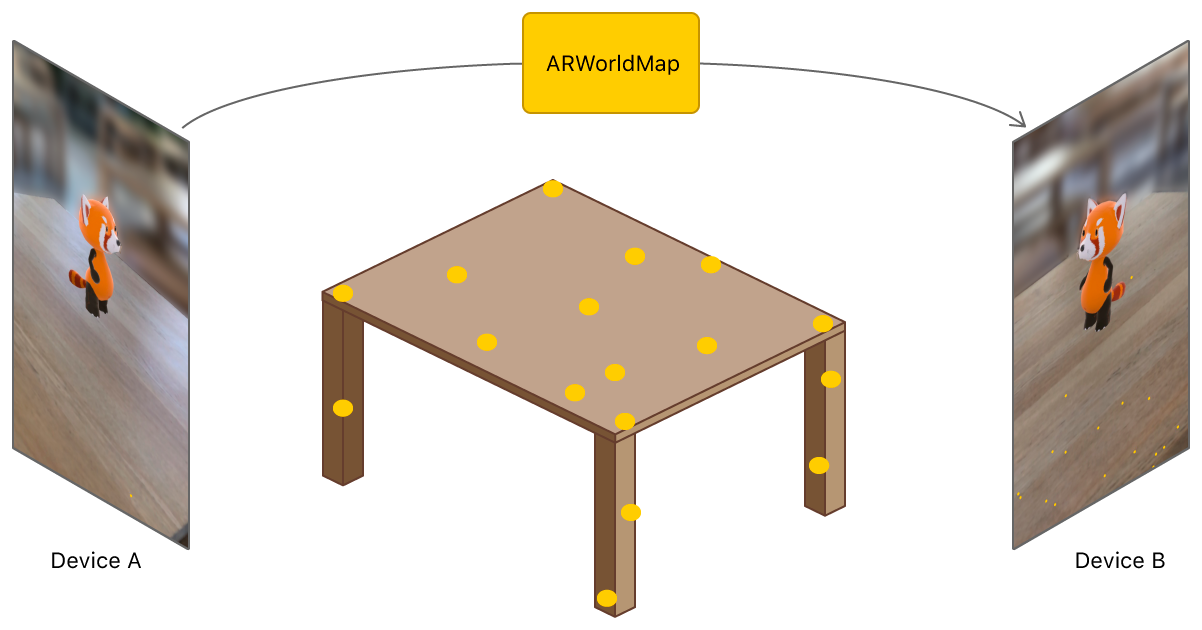
\includegraphics[width=.5\textwidth]{ar-world-map}
    \caption{ARWorldMap Synchronisierung}
    \label{ARWorldMap}
  \end{figure}

  In Abbildung \ref{ARWorldMap} ist zu sehen, wie anhand von Feature Points (gelb) die AR Session synchronisiert wird.

  \section{Wissenschaftliche Umsetzung}
  % Inwiefern wurde hier wissenschaftlich gearbeitet? Welche Forschungsfrage/n wurden geklärt und warum sind diese relevant für das Projekt?
  Für die Umsetzung des Projektes wurde die im neuen Ipad Pro erstmalig verbaute LidAR-Technologie verwendet, welche, wie bereits oben beschrieben, die Erkennung von Oberflächen und somit die Platzierung von Objekten in AR verbessert. Um herauszufinden ob die LidAR-Technologie die Immersionstiefe bei AR-Anwendungen erhöht wurden in einem User Research zehn Studenten der Hochschule Fresenius beobachtet und befragt. Die folgenden Kapitel stellen den Forschungsprozess und die Ergebnisse des User Research dar.
  \subsection{Hypothese}
  % Welche Forschungsfrage wurde gewählt und warum?
  Die von uns aufgrund der Forschungsfrage aufgestellte Hypothese lautet demnach folgendermaßen:\\

  \glqq Nutzer die eine virtuelle AR-Szene mit einem Gerät mit LidAR-Technologie betrachten haben eine bessere User Experience als Nutzer ohne LidAR. \grqq{}
  \subsection{User Research}
  % Beschreibung des durchgeführten User Research
  Für die Untersuchungen wurden die zehn Studenten der Hochschule Fresenius in zwei Gruppen aufgeteilt. Jede Gruppe sollte die App selbstständig mit einem von uns mitgebrachten Ipad testen. Dabei verfügte eins der Ipads über LidAR-Technologie und das andere nicht. Nachdem jeder Student die App selbstständig getestet hatte, wurden die Studenten gebeten jeweils zwei Fragebögen auszufüllen. Einen System Usability Scale (SUS) \cite{SUS} Fragebogen und einen AttrakDiff \cite{AttrakDiff} Fragebogen.\\ 
  Der Fragebogen zur System Usability enthält zehn Fragen um die Bedienbarkeit der App zu messen. Nutzer können bei jeder Frage zwischen \glqq Ich stimme zu\grqq, \glqq Ich stimme nicht zu\grqq{} und drei Zwischenschritten wählen.\\ 
  Der AttrakDiff Fragebogen misst die Bedienbarkeit und das Aussehen der App. Der Nutzer muss die App dabei anhand von 28 gegensätzlichen Adjektiv-Paaren bewerten und das zu der App passendere Adjektiv oder einen Zwischenwert der Adjektiv-Paare wählen.

  \subsubsection{Ergebnisse}
  \textbf{System Usability Scale}\\

  %\begin{figure}
  %\centering
  %\begin{subfigure}{.6\textwidth}
  %  \centering
  %  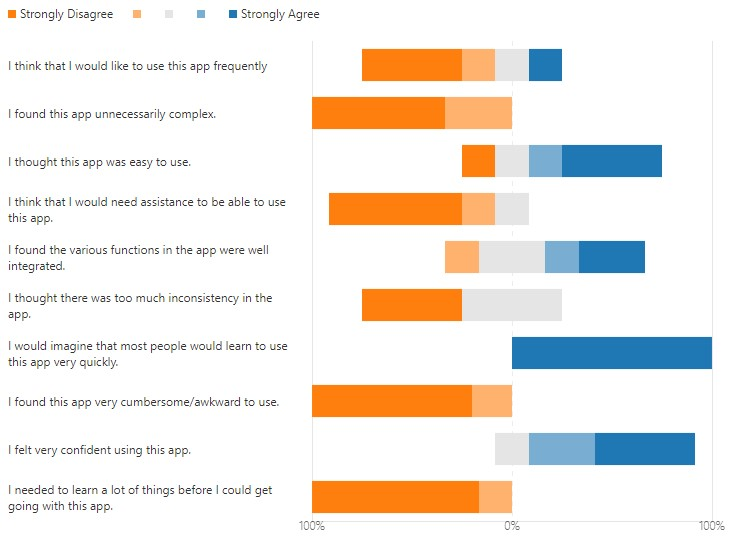
\includegraphics[width=.9\linewidth]{SUS_LiDAR}
  %  \caption{Ergebnisse mit LiDAR}
  %  \label{SUS_L}
  %\end{subfigure}%
  %\begin{subfigure}{.4\textwidth}
  %  \centering
  %  \includegraphics[width=.9\linewidth]{SUS_No_LiDAR_KF_LI}
  %  \caption{Ergebnisse ohne LiDAR}
  %  \label{SUS_NL}
  %\end{subfigure}
  %\caption{SUS Fragebogenergebnisse}
  %\label{fig:test}
  %\end{figure}

  \begin{figure}[h]
  \centering
  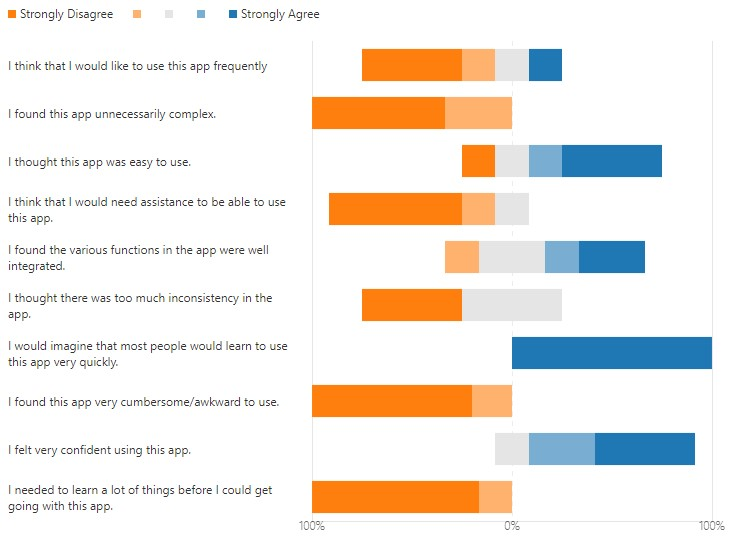
\includegraphics[width=.6\textwidth]{SUS_LiDAR}
  \caption{Ergebnisse des SUS bei Nutzern mit LiDAR}
  \label{SUS_L}
  \end{figure}

  \begin{figure}[h!]
  \centering
  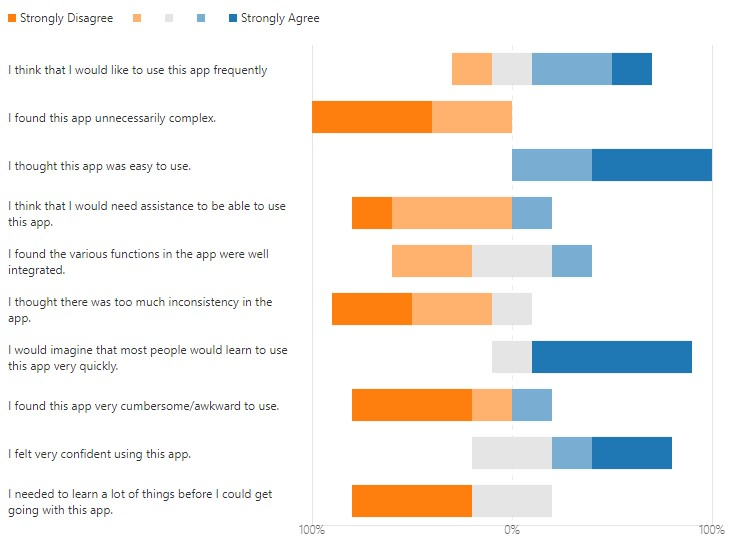
\includegraphics[width=.6\textwidth]{SUS_No_LiDAR}
  \caption{Ergebnisse des SUS bei Nutzern ohne LiDAR}
  \label{SUS_NL}
  \end{figure}

  Wie in Abbildung \ref{SUS_L} und Abbildung \ref{SUS_NL} zu sehen ähneln sich die Ergebnisse des SUS mit und ohne LiDAR Scanner sehr. Die Nutzer fanden die App sowohl mit als auch ohne LiDAR Scanner unkompliziert, leicht erlernbar, wie auch einfach und konsistent in der Benutzung. Einzig bei den Fragen ob die Nutzer die App regelmäßig nutzen würden und ob die Funktionen gut integriert seien gibt es unterschiedliche Meinungen. Die Gruppe ohne LiDAR gab an dass die Funktionen der App weniger gut integriert wären, würden die App allerdings gerne regelmäßig nutzen. Bei der Gruppe mit LiDAR Scanner gaben die Nutzer an die App nicht regelmäßig nutzen zu wollen, fanden die Funktionen der App aber gut integriert.\\

  Eine Auswertung der Fragebögen nach \cite{SUS_Score} ergab einen Wert von 79,5 für die App mit LiDAR Scanner und einen Wert von 75 ohne LiDAR Scanner. Damit erreicht die App sowohl mit als auch ohne LiDAR Scanner ein überdurchschnittliches Ergebnis nach \cite{SUS_Score}.\\

  \textbf{AttrakDiff}\\

  \begin{figure}
  \centering
  \begin{subfigure}{.5\textwidth}
    \centering
    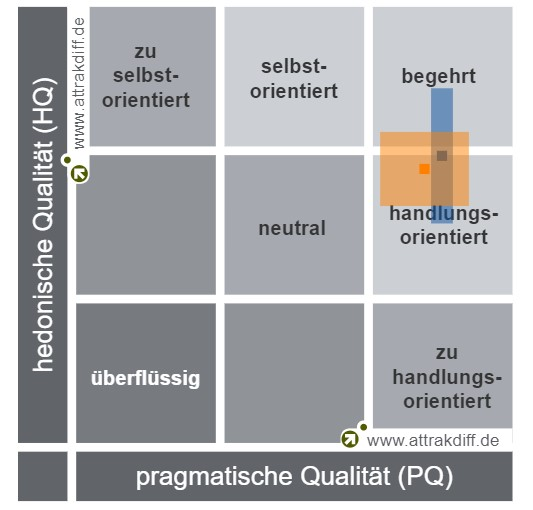
\includegraphics[width=.9\linewidth]{AttrakDiff_Portfolio}
    \caption{Portfolio der AttrakDiff Fragebogenergebnisse}
    \label{AttrakDiff_P}
  \end{subfigure}%
  \begin{subfigure}{.5\textwidth}
    \centering
    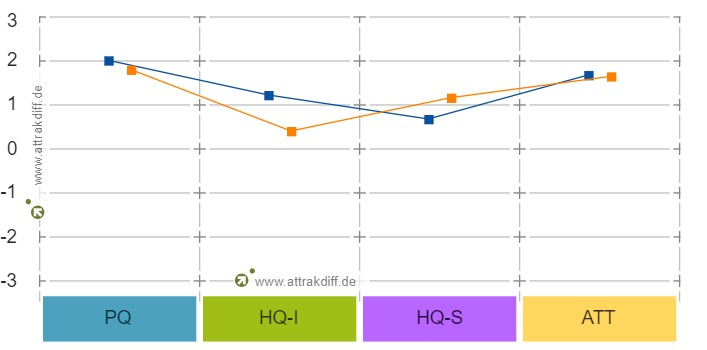
\includegraphics[width=.9\linewidth]{AttrakDiff_Mittelwerte}
    \caption{Mittelwerte der AttrakDiff Fragebogenergebnisse}
    \label{AttrakDiff_M}
  \end{subfigure}
  \caption{AttrakDiff Fragebogenergebnisse; blau: mit LiDAR; orange: ohne LiDAR}
  \label{AttrakDiff}
  \end{figure}

  Die Ergebnisse des AttrakDiff Fragebogens sind in Abbildung \ref{AttrakDiff} und Abbildung \ref{AttrakDiff_WP} zu sehen. Die Fragebogenergebnisse der Gruppe mit LiDAR und ohne LiDAR wurden dabei direkt miteinander verglichen und werden in den Grafiken farblich wie folgt dargestellt: Blau symbolisiert die Ergebnisse des Fragebogens mit LiDAR während Orange die Ergebnisse ohne LiDAR darstellt.\\
  In Abbildung \ref{AttrakDiff_P} sind die aufgestellten Portfolios der beiden Gruppen hinsichtlich hedonischer und pragmatischer Qualität zu sehen. Ein Produkt besitzt pragmatische Qualität, wenn es die Aufgabenlösung effektiv und effizient unterstützt und beziehen sich damit auf Usability im eigentlichen Sinne. Hedonische Qualität geht über die reine Nützlichkeit hinaus und beschreibt Aspekte die dem Nutzer Freude und Spaß bereiten sollen. Das Portfolio spiegelt die Angaben der Nutzer hinsichtlich der pragmatischen und hedonischen Qualität wieder. Je weiter oben im Portfolio das Produkt angeordnet ist, desto besser ist die hedonische Qualität und damit die Freude der Nutzer am Produkt. Eine Einordnung des Produktes im rechten Drittel dagegen zeugt von einem Produkt mit welchem sich die Aufgaben effizient und effektiv lösen lassen. Die Angaben der Nutzer werden in Form eines Rechtecks dargestellt. Je größer das Rechteck ist, desto unsicherer sind sich die Nutzer bezüglich der pragmatischen oder hedonischen Qualität. \\ 
  Sowohl mit als auch ohne LiDAR wurde die App als \glqq handlungsorientiert\grqq{} eingestuft, wobei die Unsicherheit bei der Gruppe ohne LiDAR hier größer ist.\\
  In Abbildung \ref{AttrakDiff_M} werden die Ergebnisse bezüglich der hedonischen Qualität weiter in Stimulation und Identität aufgeschlüsselt. Hedonische Identität bezieht sich dabei auf die Möglichkeit seine Identität durch das Produkt ausdrücken zu können und sich mit dem Produkt selber und seinem Image zu identifizieren. Die Dimension der Stimulation bildet ab, inwieweit das Produkt das Bedürfnis sich weiterzuentwickeln unterstützt, indem es neuartige, interessante und anregende Funktionalitäten, Inhalte, Interaktions- und Präsentationsstile bietet. Abbildung \ref{AttrakDiff_M} bestätigt, dass die pragmatische Qualität sowohl mit als auch ohne LiDAR mit einem Wert von ungefähr 2 überdurchschnittlich ist. Auch die Attraktivität des Produktes wird überdurchschnittlich hoch eingeschätzt. Die hedonischen Qualitäten der Identität und Stimulation sind dagegen mit einem Wert von ca. 1 eher durchschnittlich.\\
  Abbildung \ref{AttrakDiff_WP} zeigt die mittleren Ausprägungen der einzelnen Wortpaare des AttrakDiff Fragebogens. Die mittleren Ausprägungen der Wortpaare sind sowohl mit als auch ohne LiDAR sehr ähnlich. Die App wurde beide Male als einfach zu handhaben, direkt und handhabbar bewertet. Außerdem wurde die App mit dem LiDAR Scanner als sehr einbeziehend und vorzeigbar eingeschätzt. Bei der App ohne LiDAR sind diese Eigenschaften nicht so stark ausgeprägt.\\
  Ein Unterschied besteht beim herkömmlich-neuartig Adjektiv-Paar. Die App ohne LiDAR wurde als sehr neuartig eingeschätzt, während die App mit LiDAR als herkömmlich bewertet wurde.
  Abschließend wurde die App mit LiDAR als äußerst gut bewertet, ohne LiDAR fiel die Wertung etwas schlechter aus.\\
  \begin{figure}[h!]
  \centering
  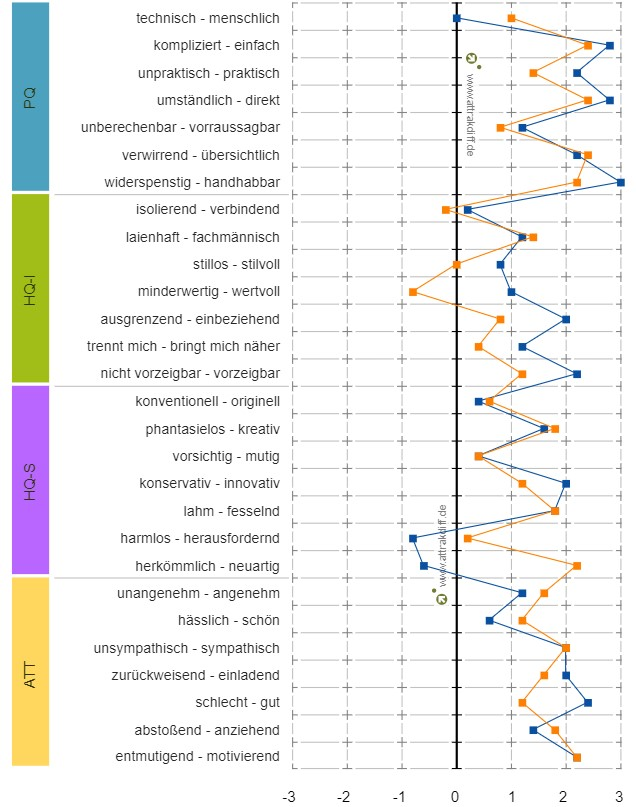
\includegraphics[width=.6\textwidth]{AttrakDiff_Wortpaare}
  \caption{AttrakDiff Wortpaare; blau: mit LiDAR; orange: ohne LiDAR}
  \label{AttrakDiff_WP}
  \end{figure}
  \subsection{Analyse der Ergebnisse}
  % Analyse der während des User Research gesammelten Daten
  Anhand der Fragebogendaten kann die Hypothese, dass LiDAR die User Experience und Immersion verbessert, nicht eindeutig bestätigt werden. Die Ergebnisse der SUS Fragebögen waren sich sehr ähnlich und auch beim AttrakDiff Fragebogen gibt es nur geringe Unterschiede. Aufgrund der Ergebnisse des AttrakDiff Fragebogens wurde die App mit LiDAR Unterstützung als ein wenig besser implementiert und vorzeigbar bewertet, allerdings gaben die Nutzer an die App ohne LiDAR regelmäßiger benutzen zu wollen.\\
  Anhand des geringen Stichprobenumfangs von fünf Personen pro Umfrage fallen individuelle Präferenzen stark ins Gewicht. Für eine aussagekräftigere Studie müssten mehr Versuchsteilnehmer befragt werden.\\

  Obwohl die Ergebnisse der Fragebögen keine stichhaltigen Ergebnisse erbrachten konnten die Aussagen der Versuchsteilnehmer während der Studie für die weitere Entwicklung nützliche Ergebnisse erbringen. Die Versuchsteilnehmer teilten uns bspw. mit dass das Scrollen der App-Auswahl nicht intuitiv sei, da die Gesten welche normalerweise auf mobilen Touchgeräten zum Scrollen verwendet werden nicht unterstützt wurden. Statt der normalen \glqq Swipe\grqq -Geste musste mit einer Scroll-Leiste an der Seite der UI gescrollt werden. Weiterhin fanden die Nutzer die Startseite der App verwirrend, da die Buttons zum Betreten der Szene als Besucher und Kurator schlecht als solche ausgezeichnet waren und einige Nutzer nicht wussten was sie tun konnten um die App zu benutzen. Eine weitere Funktionalität welche von den Nutzern erwartet wurde war das Positionieren, Rotieren und Skalieren von bereits platzierten Modellen. Die Nutzer verwendeten automatisch die hierfür erlernten Gesten und waren verwirrt und enttäuscht wenn sie feststellen mussten, dass diese keinerlei Auswirkungen haben.\\

  Neben Funktionalitäten der App welche fehlten oder noch nicht gut genug implementiert waren, teilten uns mehrere Nutzer mit, dass die App \glqq einfach zu benutzen\grqq{} und die Kern-Funktionen der App, das Auswählen und Platzieren von Modellen intuitiv verständlich sei.
  \section{Schlussfolgerungen}
  % Wie können die bei der Analyse gewonnenen Ergebnisse in das Projekt integriert werden? Bzw. wie wurden die Ergebnisse bereits integriert?
  Anhand der Ergebnisse der Fragebögen und der Auswertung der Beobachtungen der Nutzer beim Verwenden der App, sowie deren Kommentare, implementierten wir einige Änderungen am User Interface und integrierten neue, intuitiv von den Nutzern erwartete, Funktionen.\\
  Wir passten das User Interface in zweierlei Hinsicht an. Als Erstes änderten wir den Startbildschirm der App, um den Nutzern einen einfacheren Einstieg zu ermöglichen. Anstatt als Erstes den Modus, sprich Besucher oder Kurator, wählen zu müssen, wird der Nutzer nun aufgefordert einen Marker zu Scannen und kann daraufhin auswählen in welchem Modus er die Szene betritt.\\
  Um die Erwartungen der Nutzer in der App zu bedienen, änderten wir das Scroll-Verhalten der Asset-Auswahl, sodass die Nutzer wie gewohnt mit Gesten die Liste scrollen können. In diesem Zuge implementierten wir ebenfalls die von den Nutzern gewünschten Funktionen bereits platzierte Modelle später neu zu positionieren, rotieren und skalieren. Diese Funktionen wurden ebenfalls mit den von mobilen Geräten bereits bekannten Gesten implementiert.\\

  Durch die Kommentare der Nutzer und den Beobachtungen während der Nutzung konnten wir das User Interface der App deutlich verbessern und so die Nutzerzufriedenheit steigern. Die überarbeitete Version der App wurde bei späteren Demonstrationen intuitiver und besser angenommen.
  \section{Ausblick}
  % Wie könnte das Projekt in Zukunft erweitert werden?
  % PDF Unterstützung / PDFs in AR
  % AI-basierter Vorschlag ähnlicher Inhalte zum schnellen Platzieren (Quick Placement)
  % Erstellen von Lichtquellen in der AR Szene und Export der Lichtquellen als GLTF
  % Schatten
  % Integration von externen APIs wie Sketchfab oder Google Poly
  % Tutorial bei der erstmaligen Benutzung der App
  % Weitere Informationen über digitale Inhalte via dynamisch erstellter AR-Textfelder
  % Login-Maske um das Platzieren von Inhalten als Kurator zu schützen
  % Szenen direkt in der App neu erstellen und Namen ändern
  % Bilder und Videos automatisch an Wänden platzieren
  % Angepasstes App-UI für Smartphones
  Auch wenn die App bereits in einem funktionierenden Stadium ist, gibt es immer noch Features die in Zukunft ergänzt werden könnten. Die im Folgenden vorgestellten Ideen stellen eine Auswahl an Features da, welche die Nutzbarkeit der App verbessern und für einen breiteren Markt öffnen.\\
  In der App können bereits Bilder, Videos und 3D-Modelle dargestellt werden. Denkbar wäre weiterhin eine Darstellung von PDFs in AR. So könnten bspw. studentische oder wissenschaftliche Arbeiten ebenfalls virtuell ausgestellt werden.\\
  Auch wenn das Platzieren von Modellen bereits gut funktioniert, so ist die Auswahl mehrerer Modelle mühsam. Für jedes Modell muss das UI geöffnet und das gewollte Modell ausgewählt werden. Eine Verbesserung wäre hier eine durch eine AI unterstützte Schnellauswahl, welche dem User basierend auf dem gerade platzierten Modell thematisch ähnliche Modelle, z.B. aus demselben Studiengang, vorschlägt. So könnte der Workflow des Platzierens in der App erleichtert werden.\\
  Und während bei 3D-Modellen die Platzierung mitten im Raum häufig gewollt ist um das Modell von allen Seiten betrachten zu können, sind in der Luft schwebende Bilder und Videos unter Umständen nicht gewollt. Aus diesem Grund sollten zwei-dimensionale Objekte wie Bilder oder Videos automatisch an physikalischen Entitäten wie Wänden platziert werden, sodass der Eindruck entsteht die Medien würden wie in einem Museum an den Wänden hängen.\\
  Auch das Platzieren von Lichtquellen in der Szene ist geplant, um die Lichtverhältnisse in AR den Lichtverhältnissen der Realität besser anzupassen oder Highlights auf bestimmte Inhalte zu setzen. Dazu müssen Lichtquellen in AR über das App-Interface platzierbar gemacht und beim Speichern der Szene in der Datenbank gespeichert werden.\\
  Zusammen mit der Implementierung von virtuellen Lichtquellen läge die Einführung von Schatten, welche die Modelle in AR werfen, nahe. Lichtquellen und Schatten würden die virtuellen Ausstellungen noch lebendiger und realer werden lassen.\\
  Um den Informationsgehalt der virtuellen Ausstellungen zu erhöhen ist die Darstellung der Künstlerdaten, wie Name des Künstlers, Name des Modells, etc. geplant. In einem Text-UI sollen diese, bereits in der Datenbank vorliegenden, Daten dynamisch erstellt und dargestellt werden.\\
  Für die HAW Hamburg ist die Anbindung an eine, von den Studenten der HAW genutzten, Datenbank zwar sinnvoll, für andere interessierte Institutionen wie andere Hochschulen oder Museen allerdings weniger. Aus diesem Grund planen wir die Anbindung der APP an externe APIs wie Sketchfab und Google Poly, wo jeder 3D-Modelle hochladen und nutzbar machen kann. So ist die App nicht mehr nur von unserer selbst entworfenen Datenbank abhängig, sondern kann automatisch auf große Modell-Bibliotheken zugreifen.\\
  Damit von Kuratoren erstellte virtuelle Szenen nicht von Außenstehenden frei verändert werden können ist die Implementierung einer Login-Maske als Kurator in der Diskussion.\\
  Und um die Handhabung der App und das Erstellen von Szenen weiter zu vereinfachen gibt es Pläne neue Szenen direkt in der App erstellen zu können. Zur Zeit können diese ausschließlich über ein Interface auf dem CMS erstellt werden. Um diesen Schritt zu umgehen und nicht mehr von einer zweiten Application abhängig zu sein könnte dieser erste Schritt bereits in der App passieren. Weiterhin sollte der Szenen-Name direkt über die App und nicht nur über das Content-Management-System änderbar sein.\\
  Die letzten beiden Ideen handeln von einem Tutorial für Erstnutzer, welches die Funktionen der App anschaulich beim Ersten Öffnen zeigt und die Erfahrung des Nutzers so verbessert und einem angepassten Interface für Smartphones. Das jetzige Interface der App ist für das neue Ipad Pro mit LidAR-Scanner optimiert und funktioniert bei bspw. dem neuen Iphone 12 Pro nicht optimal. Eine Anpassung des User Interfaces an unterschiedliche Gerätetypen wäre bei einer wachsenden Auswahl an unterstützten Geräten wünschenswert.\\

  Wie zu sehen ist, ist das Potenzial der App bei Weitem noch nicht ausgeschöpft und wird auch in Zukunft von uns weiter entwickelt und verbessert werden. Die hier vorgestellten Features stellen unsere Ideen für eine mögliche zukünftige Erweiterung der App dar.

  \bibliographystyle{IEEEtran}
  \bibliography{literature}
\end{document}
